\documentclass{article}
\usepackage{ctex}
%\usepackage{fontspec} 
\setmainfont{Times New Roman}
\usepackage{fontspec,graphicx}
\usepackage{subfigure}
% 设置超链接
\usepackage[colorlinks,linkcolor=red]{hyperref}
\usepackage{algpseudocode}
\usepackage[linesnumbered,ruled,lined]{algorithm2e}
\usepackage{listings}
\usepackage{amsmath}


\lstset{
	columns=fixed,       
	numbers=left,                                        % 在左侧显示行号
	numberstyle=\tiny\color{gray},                       % 设定行号格式
	frame=none,                                          % 不显示背景边框
	backgroundcolor=\color[RGB]{245,245,244},            % 设定背景颜色
	keywordstyle=\color[RGB]{40,40,255},                 % 设定关键字颜色
	numberstyle=\footnotesize\color{black},           
	commentstyle=\it\color[RGB]{0,96,96},                % 设置代码注释的格式
	stringstyle=\rmfamily\slshape\color[RGB]{128,0,0},   % 设置字符串格式
	showstringspaces=false,                              % 不显示字符串中的空格
	language=TeX,                                        % 设置语言
	tabsize=2
}

\title{LaTeX用法指南} 
\author{杨涛} 
\date{5/7/2021} 

\begin{document} 

	
	\maketitle
	\tableofcontents 
	
	Hello world! 
	\section{标题1 \textbackslash section} 
	\subsection{标题2 \textbackslash subsection} 
	\subsubsection{标题3 \textbackslash subsubsection}
	
	\section{段落}
	\paragraph{段落1 \textbackslash paragraph} 
	\subparagraph{段落2 \textbackslash subparagraph}
	
	\section{正文}
	正文,
	单个换行不影响正文排版,但可以提高手稿可读性
	
	正文换行,通过两个换行符来实现换行\\也可以使用两个\textbackslash\textbackslash 来换行
	
	使用\textbackslash newpage 来开始新的一页\newpage
	我是下一页
	
	\noindent 使用\textbackslash noindent关闭缩进
	
	\section{字体设置}
	\noindent
	\tiny \textbackslash tiny 最小号\\
	\scriptsize \textbackslash scriptsize 稍小号\\
	\footnotesize \textbackslash footnotesize 角标大小\\
	\small \textbackslash small 小\\
	\normalsize \textbackslash normalsize 正常字号\\
	\large \textbackslash arge 大号\\
	\LARGE \textbackslash LARGE 更大号\\
	\huge \textbackslash huge 超大号\\
	\Huge \textbackslash Huge 最大号\\
	
	\large 
	
	\noindent\textbackslash\textnormal{textnormal}\\
	\textbackslash\textrm{textrm}\\
	\textbackslash\textsf{textsf}\\
	\textbackslash\texttt{texttt}\\
	\textbackslash\textmd{textmd}\\
	\textbackslash\textbf{textbf}\\
	\textbackslash\textup{textup}\\
	\textbackslash\textit{textit}\\
	\textbackslash\textsl{textsl}\\
	\textbackslash\textsc{textsc}\\
	\textbackslash\emph{emph}\\
	
	
	\noindent\textbackslash textcolor\{red\}\\
	\textcolor{red}{red/blue/green/black/white/cyan/magenta/yellow是系统定义颜色}\\
	\textbackslash textcolor[rgb]{0,1,0}{rgb(0, 1, 0)}
	\textcolor[rgb]{0,1,0}{rgb(0, 1, 0)}\\
	\textbackslash textcolor[RGB]{0,0,255}{RGB(0, 0, 255)}
	\textcolor[RGB]{0,0,255}{RGB(0, 0, 255)}\\
	
	\noindent 自定义颜色\\
	\begin{lstlisting}
\definecolor{myColor}{RGB}{(251, 229, 162)}
\textcolor{myColor}{我的颜色}
	\end{lstlisting}

	\definecolor{myColor}{RGB}{251, 229, 162}
	\textcolor{myColor}{我的颜色}

	
	\section{公式}
	\subsection{行内公式}
	\normalsize
	\noindent 行内公式使用\$来包裹公式,如:\$ 1 +1=\ \ \ \ 2\$\\
	这是一个行内公式$ 1 +1 =    2 $,它被嵌入到文中,公式中多余的空格不会造成副作用。
	
	\subsection{行间公式}
	\noindent 行间公式使用\textbackslash[ \textbackslash], \$\$来包裹,当然也可以使用equation来包裹
	
	\noindent 这是一个行间公式\textbackslash [1+2=3\textbackslash]\\
	\[1+2=3\] 他位于行间
	$$E=MC^2$$
	这也是个行间公式\$\$E=MC\^{}2\$\$
	\begin{equation}
		F = \frac{kQ_1Q_2}{R^2}
	\end{equation}
	\begin{lstlisting}
\begin{equation}
	F = \frac{kQ_1Q_2}{R^2}
\end{equation}
	\end{lstlisting}
	

	\subsection{上下标}
	\begin{lstlisting}
$\sum_{i=1}^{10}{a_i}$

$\int_{i=1}^{2}{x^2}$

$\prod_{i=1}^{10}{a_i}$

$\vec v$

$\overrightarrow{AB}$

$N = n_1 + n_2 + \cdots + n_m$

$ \underbrace{A+B} $

$\overline{A+B=C}$

$\underline{A+B=C}$

$  \lim_{x \to \infty} x^2_{22} - \int_{1}^{5}x\mathrm{d}x + \sum_{n=1}^{20} n^{2} = \prod_{j=1}^{3} y_{j}  + \lim_{x \to -2} \frac{x-2}{x} $

\begin{equation}
	\begin{split}
		1 = \sqrt[3]{1} \\ 
		= 1^2 \\
		= log_{10}{10}
	\end{split}
\end{equation}
	\end{lstlisting}
	
	$\sum_{i=1}^{10}{a_i}$
	
	$\int_{i=1}^{2}{x^2}$
	
	$\prod_{i=1}^{10}{a_i}$
	
	$\vec v$
	
	$\overrightarrow{AB}$
	
	$N = n_1 + n_2 + \cdots + n_m$
	
	$ \underbrace{A+B} $
	
	$\overline{A+B=C}$
	
	$\underline{A+B=C}$
	
	$ \lim_{x \to \infty} x^2_{22} - \int_{1}^{5}x\mathrm{d}x + \sum_{n=1}^{20} n^{2} = \prod_{j=1}^{3} y_{j}  + \lim_{x \to -2} \frac{x-2}{x} $
	
	\begin{equation}
		\begin{split}
		1 = \sqrt[3]{1} \\ 
		= 1^2 \\
		= log_{10}{10}
		\end{split}
	\end{equation}



	
	\subsection{大大型表达式}
	需要\textbackslash usepackage\{amsmath\}
	\subsubsection{花括号}
	
	\begin{lstlisting}
$$ f(x)=\left\{
\begin{aligned}
	x\\
	y\\
	z
\end{aligned}
\right.
$$
	\end{lstlisting}	
	
	$$ f(x)=\left\{
	\begin{aligned}
		x\\
		y\\
		z
	\end{aligned}
	\right.
	$$
	
	\begin{lstlisting}
$$
\overbrace{1+2+\cdots+n}^{n}
\quad
\underbrace{a+b+\cdots+z}_{m}
$$
	\end{lstlisting}
	
	$$
	\overbrace{1+2+\cdots+n}^{n}
	\quad
	\underbrace{a+b+\cdots+z}_{m}
	$$
	
	\subsubsection{矩阵}
	\begin{lstlisting}
\begin{equation}
	\left[
	\begin{array}{ccc}
	1 & 2 & 3\\
	4 & 5 & 6\\
	\end{array}
	\right]
\end{equation}
	\end{lstlisting}
	
	\begin{equation}
	\left[
	\begin{array}{ccc}
		1 & 2 & 3\\
		4 & 5 & 6\\
	\end{array}
	\right]
	\end{equation}
	
	\section{列表}
	\begin{lstlisting}
\begin{enumerate}
	\item 有序列表
	\begin{itemize}
		\item 无序列表
		\item[$\bullet$] 黑点
		\item[*] 星号
	\end{itemize}
	\item 有序列表
	\begin{enumerate}
		\item 套娃列表
		\item 有序列表
		\item 有序列表
	\end{enumerate}
	\item 有序列表
\end{enumerate}
	\end{lstlisting}
	\begin{enumerate}
		\item 有序列表
		\begin{itemize}
			\item 无序列表
			\item[$\bullet$] 黑点
			\item[*] 星号
		\end{itemize}
		\item 有序列表
			\begin{enumerate}
			\item 套娃列表
			\item 有序列表
			\item 有序列表
		\end{enumerate}
		\item 有序列表
	\end{enumerate}
	
	
	\section{图}
	Latex中可以插入eps、png、pdf、jpg等格式的图
	SVG需要用AI或者InkScape转为EPS或者PDF再插入
	%\usepackage{graphicx}
	
	单栏
	\begin{lstlisting}
\begin{figure}
	\centering
	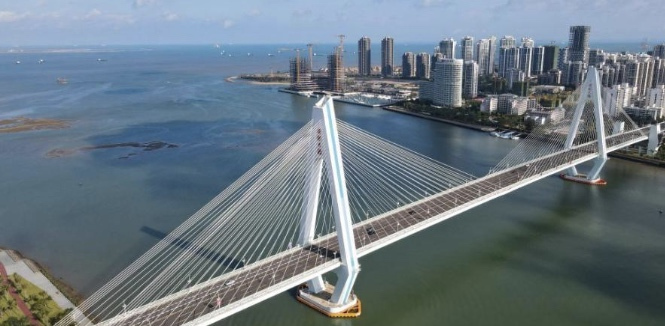
\includegraphics[width=0.7\linewidth]{fig1.jpg}
	\caption{这里是图注}
	\label{fig:fig1}
\end{figure}
	\end{lstlisting}
	
	\begin{figure}
		\centering
		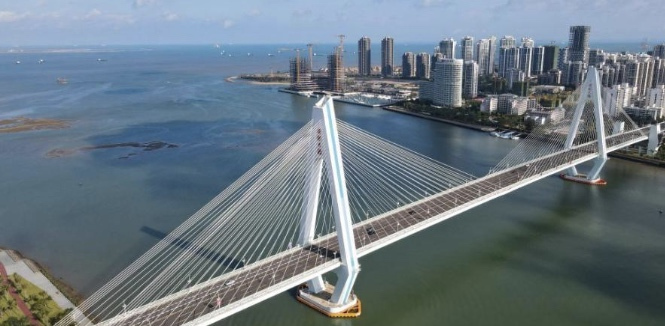
\includegraphics[width=0.7\linewidth]{fig1.jpg}
		\caption{这里是图注}
		\label{fig:fig1}
	\end{figure}
	
	双栏
	\begin{lstlisting}
\begin{figure}
	\centering
	\subfigure[fig1 caption]{
		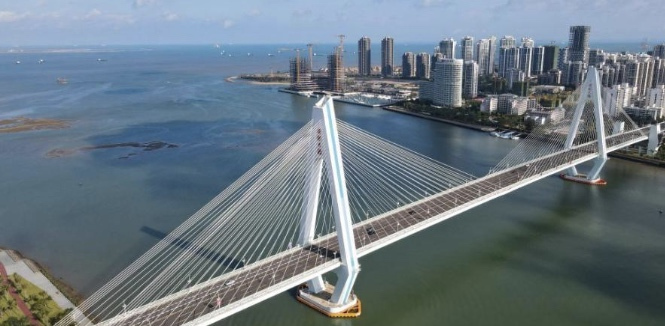
\includegraphics[width=0.4\linewidth]{fig1.jpg}
		\label{fig:fig2}
	}
	\subfigure[fig2 caption]{
		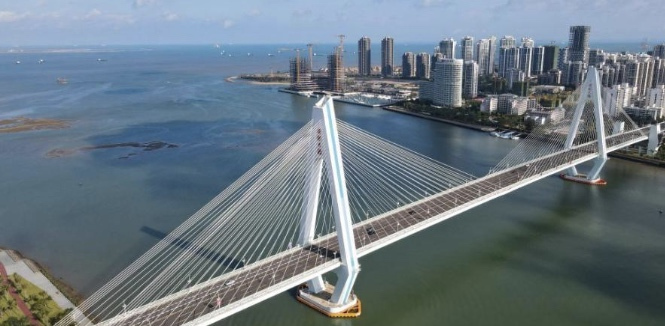
\includegraphics[width=0.4\linewidth]{fig1.jpg}
		\label{fig:fig3}
	}
	\caption{题注}
	\label{fig:figset}
\end{figure}
	\end{lstlisting}
	
	
	%\usepackage{subfigure}
	\begin{figure}
		\centering
		\subfigure[fig1 caption]{
			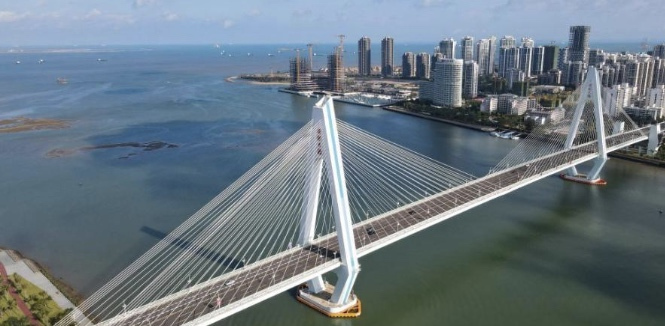
\includegraphics[width=0.4\linewidth]{fig1.jpg}
			\label{fig:fig2}
		}
		\subfigure[fig2 caption]{
			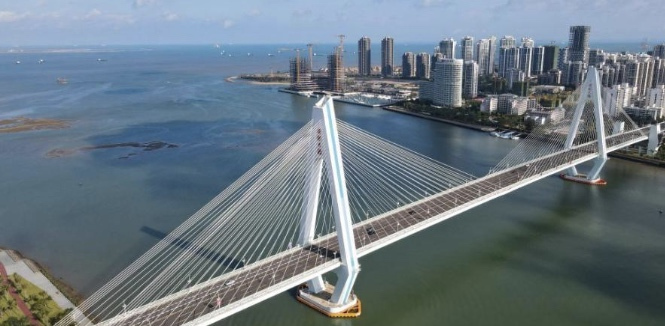
\includegraphics[width=0.4\linewidth]{fig1.jpg}
			\label{fig:fig3}
		}
		\caption{题注}
		\label{fig:figset}
	\end{figure}
	
	\section{绘图}
	与SVG的绘图方式相似,LaTeX可以使用坐标来进行绘图
	\begin{lstlisting}
\begin{picture}(50,50)
	\thicklines\qbezier(0,0)(0,50)(50,50)
	\qbezier[20](0,0)(50,0)(50,50)
	\thinlines
	\put(0,0){\line(1,1){50}}
\end{picture}	
	\end{lstlisting}
	\begin{picture}(50,50)
		\thicklines\qbezier(0,0)(0,50)(50,50)
		\qbezier[20](0,0)(50,0)(50,50)
		\thinlines
		\put(0,0){\line(1,1){50}}
	\end{picture}
	
	\section{引用}
	\begin{lstlisting}
图\ref{fig:fig1}显示了。 。。图\ref{fig:fig2}。。。
	\end{lstlisting}
	
	图\ref{fig:fig1}显示了。 。。图\ref{fig:fig2}。。。
	
	
	\section{脚注}
	\begin{lstlisting}
这是一个脚注\footnote{我是脚注内容}	
	\end{lstlisting}
	这是一个脚注\footnote{我是脚注内容}
	
	\section{超链接}
	\begin{lstlisting}
这是一个超链接指向\href{www.baidu.com}{百度}
这是百度的url\url{www.baidu.com}
	\end{lstlisting}
	这是一个超链接指向\href{www.baidu.com}{百度}
	这是百度的url\url{www.baidu.com}
	
	\section{表格}
	\begin{lstlisting}
\begin{table}
	\caption{表头}
	\label{tab:table1}
	\begin{tabular}{p{45pt} p{55pt} p{55pt} p{55pt} p{55pt}}
		\hline\noalign{\smallskip}
		A & B & C & MAE & D \\
		\noalign{\smallskip}\hline\noalign{\smallskip}
		1 & 2.07 & 4.55\% & 739.83 & 2.73%\\
		3 & 1.66 & 6.62\% & 1131.90 & 3.82%\\
		7 & 2.49 & 11.31\% & 5726.90 & 18.05%\\
		\noalign{\smallskip}\hline
	\end{tabular}
\end{table}
	\end{lstlisting}
	\begin{table}
		\caption{表头}
		\label{tab:table1}
		\begin{tabular}{p{45pt} p{55pt} p{55pt} p{55pt} p{55pt}}
			\hline\noalign{\smallskip}
			A & B & C & MAE & D \\
			\noalign{\smallskip}\hline\noalign{\smallskip}
			1 & 2.07 & 4.55\% & 739.83 & 2.73\%\\
			3 & 1.66 & 6.62\% & 1131.90 & 3.82\%\\
			7 & 2.49 & 11.31\% & 5726.90 & 18.05\%\\
			\noalign{\smallskip}\hline
		\end{tabular}
	\end{table}
	
	\section{伪代码}
	%\usepackage{algpseudocode}
	%\usepackage{amsmath}  
	%\usepackage{algpseudocode} 
	
	\begin{algorithm}[htbp]{
	\caption{标题}
		\label{alg:mss}
		\KwIn {$target:$\ Recent trends in the target area
			\\ \qquad \quad \ \ $simi(m,\ n):$\ Calculate the distance between sequence $m$ and $n$
			\\ \qquad \quad \ \ $S:$\ Outbreak data sequences for other regions}
		\KwOut{$A:$\ The shortest distance from the $target$ in the sequence of each region}
		Initialize $A = \emptyset$\;
		$t \gets $the\ length\ of\ sequence$\ target$\;
		\leavevmode \\
		$target \gets $Normalize$\ target$\;
		$S \gets $Normalize\ the\ sequence\ in$\ S$\;
		/* $s_i\ $Represents\ the\ pandemic\ data\ sequence\ of\ the$\ i_{th}\ $area\ in$\ S$ */\;
		\For {$s \in \{s_1,s_2,...\}$}
		{
			$ls \gets $the\ length\ of\ sequence$\ s$\;
			\For {$i = 0\ \rm{to}\ ls$}
			{
				\If{$simi$\ \rm{requires\ the\ two\ sequences\ to\ be\ equal\ in\ length}}{
					\For{$j = i$\ \rm{to}\ $(ls - t)$}{
						$d \gets simi(target,s[i,\ j])$\;
					}
				}
				\Else{
					/* Consider sequences of different lengths */\;
					\For{$f = 0$\ \rm{to}\ $2t$}{
						\For{$j = i$\ \rm{to}\ $(ls - f)$}{
							$d \gets simi(target,s[i,\ j])$\;
						}
					}
				}
			}
			$D,I,J \gets $When $d$ gets the maximum value, the values of $d,\ i\ $and$\ j$, respectively\;
			add $(D,\ s[i,j])\ \rm{to}\ A$\;
		}
		Sort the elements in $A$ in descending order according to the value of $D$\;
			\Return{$A$}\;
		}
	\end{algorithm}
	
	\section{参考文献}
	参考文献只会显示文中引用的部分
	
	\subsection{不通过BibTex}
	\textbackslash begin{thebibliography}{num} : num定义了最大文献数量
	每一条参考文献使用\textbackslash bibitem{引用标志}文献导出
	通过\textbackslash cite{引用标志}来引用文献\cite{ref666}
	\begin{lstlisting}
\begin{thebibliography}{10} 
	\bibitem{ref1}杨涛.这是一条参考文献[J].Viva525,2021,1(1):1-2.
	\bibitem{ref666}杨涛.这又是一条参考文献[J].Viva525,2021,1(1):1-2.
\end{thebibliography}
	\end{lstlisting}
	\begin{thebibliography}{10} 
		\bibitem{ref1}杨涛.这是一条参考文献[J].Viva525,2021,1(1):1-2.
		\bibitem{ref666}杨涛.这又是一条参考文献[J].Viva525,2021,1(1):1-2.
	\end{thebibliography}

	\subsection{使用BibTeX}
	在文末插入标记,ref是文件名,可以自定义\cite{lgz}
	
	\noindent\textbackslash bibliographystyle\{plain\}\\
	\textbackslash bibliography\{ref\} 
	
	常见的预设样式的可选项有8种,分别是:
	
	plain,按字母的顺序排列,比较次序为作者、年度和标题;
	
	unsrt,样式同plain,只是按照引用的先后排序;
	
	alpha,用作者名首字母+年份后两位作标号,以字母顺序排序;
	
	abbrv,类似plain,将月份全拼改为缩写,更显紧凑;
	
	ieeetr,国际电气电子工程师协会期刊样式;
	
	acm,美国计算机学会期刊样式;
	
	siam,美国工业和应用数学学会期刊样式;
	
	apalike,美国心理学学会期刊样式;
	
\bibliographystyle{plain}
\bibliography{ref.bib}
\end{document}